% !TeX spellcheck = en_GB

\section{Proofs and Mathematical Detail for Chapter~4}
\label{app:temporal_tuning_proofs}

This section contains proofs for the mathematical claims made throughout \Cref{chp:temporal_tuning}.
Specifically, we prove that our least-squares loss generalises the \NEF dynamics principle, that our notion of a \enquote{delay re-encoder} works as intended, and provide the complete derivation of the \LDN system using the delay re-encoder.

\subsection{Proof for Theorem~4.1}
\label{app:lstsq_nef_equivalence}

We claimed in \Cref{sec:temporal_tuning_lti} that solving our least-squares loss function in linear networks with homogeneous first-order low-pass filters results in exactly the same solution as using the \NEF dynamics principle.
More precisely, we claimed the following:

\thmTemporalLstsq*

\begin{proof}
We prove this theorem in two steps: \emph{(1)} the solution to the least-squares loss is indeed unique, and \emph{(2)} we can achieve a zero error with the solution mentioned above; therefore, this solution must be the global optimum.
Note that the first part of our proof is less rigorous; we pay less attention to some edge-cases that could technically occur.

\paragraph{(1) The solution to the least-squares loss is unique}
We have a linear least-squares loss over $n + 1$ variables and $N \geq n + 1$ samples.
For a unique solution, the design matrix $\mat P \in \mathbb{R}^{N \times {n + 1}}$ must be of full column rank:
\begin{align*}
	\mat P =
	\NiceMatrixOptions{renew-dots,renew-matrix}
	\begin{bmatrix}
			(h \ast \mathfrak{x}_1)(0)
		&	(h \ast (\mathfrak{e}_1 \ast \mathfrak{x}_1))(0)
		&	\ldots
		&	(h \ast (\mathfrak{e}_n \ast \mathfrak{x}_1))(0) \\
			(h \ast \mathfrak{x}_2)(0)
		&	(h \ast (\mathfrak{e}_1 \ast \mathfrak{x}_2))(0)
		&	\ldots
		&	(h \ast (\mathfrak{e}_n \ast \mathfrak{x}_2))(0) \\
		\vdots & \vdots & \ddots & \vdots\\
			(h \ast \mathfrak{x}_N)(0)
		&	(h \ast (\mathfrak{e}_1 \ast \mathfrak{x}_N))(0)
		&	\ldots
		&	(h \ast (\mathfrak{e}_n \ast \mathfrak{x}_N))(0)
	\end{bmatrix}
\end{align*}
where \enquote{$\ast$} denotes convolution.
Because all functions $\mathfrak{e}_i$ and $\mathfrak{x}_k$ are pairwise linearly independent, $\mat P$ is usually of full column rank; filtering each function with the same low-pass filter $h$ does not change this.
One possible exception would be selecting pathological $\mathfrak{x}_k$ that are orthogonal to all $\mathfrak{e}_k$; random $\mathfrak{x}_k$ are unlikely to have this property.

\paragraph{(2) Using the matrices $\mat A'$ and $\mat B'$ as a solution results in a zero error}
Instead of proving this for the input sequences $\mathfrak{x}_k$, we instead prove this property for any $\mathfrak{x}$.
In particular, for a zero error in the least-squares loss, the following equality most hold for all $i \in \{1, \ldots, n\}$.
\begin{align*}	
	\int_{0}^\infty \!\! \mathfrak{e}_i(\tau) \mathfrak{x}(-\tau) \mathrm{d}\tau
	&\supposedEq \,
	\int_0^\infty \!\! b'_{i} h(\tau) \mathfrak{x}_k(-\tau) + \sum_{j=1}^n a'_{ij} h(\tau) \int_0^\infty \!\! \mathfrak{x}_k(-\tau - \tau') \mathfrak{e}_j(\tau') \, \mathrm{d}\tau' \mathrm{d}\tau  \,.
\end{align*}
Rewriting the integrals as convolutions evaluated at zero and rearranging, we obtain
\begin{align*}	
	0
	&\supposedEq \, (\mathfrak{e}_i \ast \mathfrak{x})(0) - b'_{i} (h \ast \mathfrak{x})(0) - \sum_{j=1}^n a'_{ij} (h \ast (\mathfrak{e}_n \ast \mathfrak{x}))(0) \,.
\end{align*}
Expressing the convolution operations vectorially over all $i$ in the Laplace domain (evaluating the convolution everywhere, and not just at zero), we get
\begin{align}
	0 &\supposedEq \,  E(s) X(s) - \mat B' H(s) X(s) - \mat A' H(s) E(s) X(s) \,.
	\label{eqn:temporal_tuning_opt_laplace}
\end{align}
Per definition, $E(s)$ is the impulse response of the \LTI system defined by $\mat A$, $\mat B$.
Let $M(s)$ be the Laplace transform of the linear system state $\vec m(t)$.
We have the following quantities:
\begin{align*}
	M(s) &= \frac{1}{s} \mat A M(s) + \mat B X(s) \,,
	& E(s) &= \frac{M(s)}{X(s)} = \frac{1}s \frac{\mat A M(s) + \mat B X(s)}{X(s)} \,.
\end{align*}
Furthermore, recall that the first-order low-pass filter $H(s)$ is given as
\begin{align*}
	H(s) &= \frac{1}{\tau s + 1} \,.
\end{align*}
Substituting these definitions along with $\mat A' = \tau \mat A + \mat I$ and $\mat B' = \tau \mat B$ into \cref{eqn:temporal_tuning_opt_laplace} yields
\begin{align*}
	&\hphantom{{}={}} E(s) X(s) - \mat B' H(s) X(s) - \mat A' H(s) E(s) X(s) \\
	&= \frac{1}{s} \bigl( \mat A M(s) + \mat B X(s) \bigr)
	 - \mat B' H(s) X(s)
	 - \frac{1}{s} \mat A' H(s) \bigl(\mat A M(s) + \mat B X(s)\bigr) \\
	&= \frac{1}{s} \bigl( \mat A M(s) + \mat B X(s) \bigr)
	 - \frac{1}{\tau s + 1} \mat B' X(s)
	 - \frac{1}{(\tau s + 1) s} \mat A' \bigl( \mat A M(s) + \mat B X(s) \bigr) \\
	&= \frac{1}{s} \bigl( \mat A M(s) + \mat B X(s) \bigr)
	 - \frac{1}{\tau s + 1} \tau \mat B X(s)
	 - \frac{1}{(\tau s + 1) s} \bigl(\tau \mat A + \mat I \bigr) \bigl(\mat A M(s) + \mat B X(s)\bigr) \\
	&= \frac{\bigl(\mat A M(s) + \mat B X(s) - s M(s)\bigr) \mat A \tau}{(\tau s + 1) s} \\
	&= \frac{\bigl(\mat A M(s) + \mat B X(s) - \mat A M(s) - \mat B X(s)\bigr) \mat A \tau}{(\tau s + 1) s} \\
	&= 0 \,. \qedhere
\end{align*}
\end{proof}

\pagebreak

\subsection{Temporal Tuning and Nonlinear Dynamics}
\label{app:temporal_tuning_nonlinear}

We noted that temporal tuning is a generalisation of the \NEF dynamics principle.
That is, we can---in addition to accounting for heterogeneous and higher-order filters, and taking empirical data into account---use temporal tuning curves to implement any dynamical system that could be implemented using the dynamics principle.
This includes nonlinear dynamical systems.

%Below, we first review realising nonlinear dynamics in \NEF networks, and then, using the same argument as in our proof of \Cref{thm:temporal_lstsq} (cf.~\Cref{app:lstsq_nef_equivalence}), discuss why solving for weights using nonlinear temporal tuning curves must result in the same solution.

\subsubsection{Nonlinear dynamical systems in the \NEF}

\begin{figure}
	\centering
	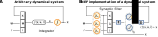
\includegraphics{media/chapters/ZB_details/nef_dyn_sys.pdf}%
	{\phantomsubcaption\label{fig:nef_dyn_sys_a}}%
	{\phantomsubcaption\label{fig:nef_dyn_sys_b}}%
	\caption[Implementing arbitrary nonlinear dynamics in the NEF]{
		Implementing arbitrary nonlinear dynamics in the \NEF.
		\textbf{(A)} Diagram illustrating integrating an arbitrary dynamical system. The state $\vec x$, input $\vec u$ and time $t$ are passed through $f$ to obtain the differential $\dot{\vec x}$. The integral of $\dot{\vec x}$ is equal to $\vec x$.
		\textbf{(B)} Implementing the same system in the \NEF. All quantities are passed through a first-order low-pass filter with time-constant $\tau$.
		The output of the filter operation is then represented in a population of neurons using an encoder matrix $\mat E$ in a population of $n$ neurons. We can then decode the feedback function $f'$ compensating for the synaptic filter. The state $\vec x$ is exactly the result of passing the result of $f'$ through the low-pass filter.
	}
	\label{fig:nef_dyn_sys}
\end{figure}

\Cref{thm:temporal_lstsq} states that, under some mild conditions, our optimisation problem in \cref{eqn:weight_optimise_currents_temporal_no_trafo} perfectly realises any \LTI system of the form $\dot{\vec m}(t) = \mat A \vec m(t) + \mat B \vec u(t)$ in a recurrently connected linear neuron population, given that the connecting synapses are heterogeneous first-order low-pass filters.
In particular, the resulting weight matrices are $\mat A' = \tau \mat A + \mat I$, and $\mat B' = \tau \mat B$.
These matrices implement the desired \LTI system while compensating for the low-pass filter acting as a leaky integrator (cf.~\Cref{fig:nef_dynamics_ab}).
%This is exactly the relationship pointed out by \Citet[Chapter~8]{eliasmith2003neural} as part of the original description of the \NEF dynamics principle.

While this is an important observation, the \NEF dynamics principle is more general than that.
As we noted in \Cref{sec:nef_dynamics}, the above substitution is a special case of a more general transformation that can be used to implement any dynamical system of the form $\dot{\vec x}(t) = f(\vec x(t), \vec u(t), t)$ across a low-pass filter with time-constant $\tau$ (cf.~\Cref{fig:nef_dyn_sys}).
We have:
\begin{align}
	f'(\vec x(t), \vec{\hat u}(t), \hat t(t)) = \tau f(\vec x(t), \vec{\hat u}(t), \hat t(t)) + \vec x(t) \,.
	\label{eqn:nef_dynamics_general}
\end{align}
Here, $\vec{\hat u}(t)$ and $\hat t(t)$ are low-pass filtered versions of the input and the time $t$.
Note that this is a \emph{perfect} transformation.
As long as we are able to realise $f'$ without error, the resulting system will perfectly produce the desired dynamics described by $f(\vec x(t), \vec u(t), t)$.
Of course, to realise an arbitrary $f'$ that is nonlinear over $\vec x(t)$, $\vec{\hat u}(t)$, $\hat t(t)$, all these variables must be represented in a single neuron population with diverse tuning (cf.~\Cref{fig:nef_dyn_sys_b}).

\subsubsection{Nonlinear temporal tuning curves}

To realise nonlinear dynamical systems using the temporal tuning paradigm, we need to make use of the general concept of a temporal tuning curve from \Cref{def:temporal_tuning_curve}; \emph{linear} temporal tuning curves (\Cref{def:linear_temporal_tuning}) are restricted to \LTI systems.
For the sake of simplicity, we only consider time-invariant systems, that is $f(\vec x, \vec u)$.%
\footnote{
The same considerations of course still hold if we supply an external time variable, for example as part of $\mathfrak{u}$.
Technically, neither the temporal tuning approach, nor the \NEF are truly capable of realising time-variant systems. The universal approximator properties of two-layer networks only hold for compact domains $\mathbb{X}$ (cf.~\Cref{thm:two_layer_universal}); as soon as time is represented, $\mathbb{X}$ is no longer compact. In practice, $t$ could be compressed into a vector representation using Spatial Semantic Pointers \citep{komer2020biologically}.}

The temporal tuning curve of a neuron tuned to an $n$-dimensional system $f(\vec x, \vec u)$ is
\begin{align*}
	a_i(\mathfrak{u}) &=
		G\Bigl[ \alpha_i \bigl\langle \vec e_i, \bigl(\vec x(0, \mathfrak{u}), (h \ast \mathfrak{u})(0) \bigr) \bigr\rangle + \beta_i \Bigr] \,,
		& \quad \text{where} \quad
			\vec x(t, \mathfrak{u}) &=  \int_{-\infty}^t f(\vec x(t', \mathfrak{u}), \mathfrak{u}(t')) \,\mathrm{d}t' \,.
\end{align*}
Here, $a_i$ is the activity of the $i$th neuron given an $m$-dimensional input signal $\mathfrak{u} : \mathbb{R}^- \longrightarrow \mathbb{R}^m$, and $\vec e_i$ is an encoding vector uniformly sampled from the hypersphere $\mathbb{S}^{m + n}$.
This tuning curve exactly describes the activity of a neuron in \Cref{fig:nef_dyn_sys_b} in response to an input signal $\mathfrak{u}$.

With this temporal tuning, in the limit of an infinite number of neurons $m \to \infty$ and samples $N \to \infty$, and w.l.o.g. $J_i(\xi) = \xi$, our optimisation problem from \cref{eqn:weight_optimise_currents_temporal_no_trafo} becomes
\begin{align*}
	E &= \sum_{k = 1}^N \left[
			\bigl\langle \vec e_i, \bigl(\vec x(0, \mathfrak{u}_k), (h \ast \mathfrak{u}_k)(0) \bigr) \bigr\rangle \,-\,
			\sum_{j = 1}^m w_{ij} \! \int_0^\infty \!\!\! h(\tau) a_j(\mathfrak{u}_k \ast \delta_\tau) \,\mathrm{d}\tau \,-\,
			\sum_{j = 1}^m w'_{ij} (h \ast \mathfrak{u}_k)(0)
		\right]^2 \,,
\end{align*}
where the $w_{ij}$ are the feedback weights, and the $w'_{ij}$ are the input weights.
Obviously, the optimal input weights $w'_{ij}$ are merely a block of the encoder matrix $\mat E$.
This leaves us with determining the feedback weights $w_{ij}$.
In particular, note that it must hold $E = 0$ if we can find a decoding matrix $(\mat D)_{ij} = d_{ij}$ such that for all $k$ and all $i \in \{1, \ldots, n\}$
\begin{align*}
	\bigl(\vec x(0, \mathfrak{u}_k)\bigr)_i = \sum_{j = 1}^m d_{ij} \! \int_0^\infty \!\!\! h(\tau) a_j(\mathfrak{u}_k \ast \delta_\tau) \,\mathrm{d}\tau = \sum_{j = 1}^m \! \int_0^\infty \!\!\! h(\tau) d_{ij} a_j(\mathfrak{u}_k \ast \delta_\tau) \,\mathrm{d}\tau \,.
\end{align*}
Since $m, N \to \infty$, and our neuron population represents the current state $\vec x = \vec x(0, \mathfrak{u}_k)$ and the low-pass filtered input $\vec{\hat u}$, we can further simplify this to:
\begin{align*}
	(\vec x )_i = \int_0^\infty \!\!\! h(\tau) f'_i(\vec x(-\tau), \vec{\hat u}(-\tau)) \,\mathrm{d}\tau \,.
\end{align*}
In other words, the optimal solution is a function $f'$ that takes $\vec x$, the filtered $\vec{\hat u}$, and, if being passed through a first-order low-pass filter $h$ over time, returns the current state $\vec x$.
Our $f'$ from above \emph{exactly} fulfills this property (cf.~\Cref{fig:nef_dyn_sys_b}); hence, by the same argument as in our proof for \Cref{thm:temporal_lstsq} (and under the same mild conditions), the optimisation problem \emph{must} solve for connection weights that realise $f'$.

\clearpage

\subsection{Heterogeneous Time Constants Require Access to the Derivative}
\label{app:heterogenous_time_constants}

\begin{figure}
	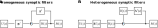
\includegraphics{media/chapters/ZB_details/homogeneous_heterogeneous_filters.pdf}%
	{\phantomsubcaption\label{fig:homogeneous_heterogeneous_filters_a}}%
	{\phantomsubcaption\label{fig:homogeneous_heterogeneous_filters_b}}%
	\caption[Block-diagram of a recurrent networks with homogeneous and heterogeneous filters]{Block-diagram of a recurrent networks with homogeneous and heterogeneous filters in the Laplace domain. $U(s)$ is the input signal, $M(s)$ is the state vector with the desired \LTI dynamics $s M(s) = \mat A M(s) + \mat B U(s)$.
	\textbf{(A)} Recurrent network used in the derivation of the \NEF dynamics principle. The input and feedback pass through the same filter $H(s)$.
	This filter takes the role of the integrator in a standard \LTI system; $\mat A'$ and $\mat B'$ compensate for the lack of an integrator to realise the desired dynamics.
	\textbf{(B)} For heterogeneous $H_1(s)$, $H_2(s)$, both $\mat A'(s)$ and $\mat B'(s)$ are time-dependent filters themselves.
	}
	\label{fig:homogeneous_heterogeneous_filters}
\end{figure}

We mentioned in \Cref{sec:lti_complex_networks} that compensating for the dynamics of a network with heterogeneous time-constants requires access to the derivative of the input and feedback signal.
To get some intuition for this, recall the derivation of the original \NEF dynamics principle (cf.~\Cref{sec:nef_dynamics}; \cite{eliasmith2003neural}, Chapter~8).
Using the homogeneous network illustrated in \Cref{fig:homogeneous_heterogeneous_filters_a}
\begin{align}
	M(s) &= \frac{1}{s} \bigl( \mat A M(s) + \mat B U(s) \bigr) \,, \label{eqn:desired_dyn}\\
	\text{and} \quad\quad M(s) &= \mat B' H(s) U(s) + \mat A' H(s) M(s) = \frac{1}{\tau s + 1} \bigl( \mat B' U(s) + \mat A' M(s) \bigr) \label{eqn:homo_dyn}\,,
\end{align}
where the first line are our desired dynamics, and the second line are the actual network dynamics.
Multiplying both sides of \cref{eqn:homo_dyn} with $\tau s + 1$ and rearranging the equation into the form of \cref{eqn:desired_dyn} and solving for $\mat A'$, $\mat B'$ yields:
\begin{align*}
	M(s) &= \frac{1}{s} \left( \frac{\mat A' - \mat I}{\tau} M(s) +  \frac{\mat B'}{\tau}  U(s) \right) \quad\quad \Rightarrow \quad\quad \mat A' = \tau \mat A + \mat I \,, \quad \mat B' = \tau \mat B \,.
\end{align*}

We can now repeat the same procedure for the network with heterogeneous synaptic filters depicted in \Cref{fig:homogeneous_heterogeneous_filters_b}; however, we will obtain filters $\mat A'(s)$, $\mat B'(s)$.
Assuming that $H_1(s)$ and $H_2(s)$ are first-order low-pass filters with time-constants $\tau_1$, $\tau_2$, we have
\begin{align*}
	M(s) &= \mat B'(s) H_1(s) U(s) + \mat A'(s) H_2(s) M(s) = \mat B'(s) \frac{1}{\tau_1 s + 1} U(s) + \mat A'(s) \frac{1}{\tau_2 s + 1} M(s) \,.
	\label{eqn:hetero_dyn}
\end{align*}
To make sure that our filters $\mat A'(s)$ and $\mat B'(s)$ are causal (i.e., the order of the numerator is smaller or equal to the order of the denominator), we must first rearrange the equation, for example after multiplying both sides with $(\tau_1 s + 1) (\tau_2 s + 1)$.
We obtain
\begin{align*}
	M(s) &= \frac{1}{s} \left(
		  \frac{ \mat A'(s) (\tau_1 s + 1) - \mat I ((\tau_1 + \tau_2) s - 1 )}{s \tau_1 \tau_2} M(s)
		+ \frac{\mat B'(s) (s \tau_2 + 1)}{s \tau_1 \tau_2} U(s)
	\right) \,.
\end{align*}
Solving for $\mat A'(s)$ and $\mat B'(s)$ results in two first-order high-pass filters:
\begin{align*}
	\mat A'(s) &= \frac{(\mat A \tau_1 \tau_2 + \tau_1 + \tau_2) s + 1}{\tau_1 s + 1} \,, &
	\mat B'(s) &= \frac{\mat B \tau_1 \tau_2 s}{\tau_2 s + 1} \,.
\end{align*}
Curiously, this solution does not coincide with the original \NEF solution for $\tau_1 = \tau_2$; this is due to the problem of finding $\mat A'(s)$ and $\mat B'(s)$ being underconstrained.
However, and without providing a proof, for $\tau_1 \neq \tau_2$, $s$ will always be in the numerator of $\mat A'(s)$ and $\mat B'(s)$; correspondingly, these filters require access to the derivative of their input.

\subsection{Homogeneous Recurrent Networks with Interneurons}
\label{app:granule_golgi_dynamics}

\begin{figure}
	\centering
	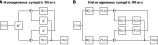
\includegraphics{media/chapters/ZB_details/intermediate_population_filters.pdf}
	{\phantomsubcaption\label{fig:intermediate_population_filters_a}}%
	{\phantomsubcaption\label{fig:intermediate_population_filters_b}}%
	\caption[Block-diagram of recurrent networks with an interneuron population]{Block-diagram of the dynamics of a recurrent network with an interneuron population. As in \Cref{fig:homogeneous_heterogeneous_filters}, $U(s)$ is the input signal, $M(s)$ is the state vector with desired dynamics $s M(s) = \mat A M(s) + \mat B U(s)$.
	\textbf{(A)} If all synaptic filters in the feedback and inhibitory path are the same, then there is a simple time-invariant solution for matrices $\mat A'$, $\mat B'$ that realise the dynamical system.
	\textbf{(B)} For heterogeneous filters, there is no time-invariant solution for the input and feedback matrices. See \Cref{sec:lti_complex_networks} for a numerical approximation.}
\end{figure}

We claimed in \Cref{sec:lti_complex_networks} that the time-invariant matrices $\mat A' = \tau \mat A + \mat I$, $\mat B' = \tau \mat B$ can be used to realise any desired \LTI system in a recurrent neural network with an intermediate population and homogeneous synaptic filters (cf.~\Cref{fig:intermediate_population_filters_a}).
We discuss why this is the case below---we first provide an intuitive solution, and then prove the result more rigorously.
Note that, similarly to the argument made in the previous section, finding time-invariant $\mat A'$, $\mat B'$ is generally not possible for recurrent networks with heterogeneous filters (cf.~\Cref{fig:intermediate_population_filters_b}).

\paragraph{Intuitive explanation}
Observe that if we were able to \enquote{undo} the filtering performed by the synaptic filter of the upper interneuron population, we would have a \enquote{normal} recurrent neuron population. In other words, we would, from the perspective of the \enquote{primary} neuron like interneurons to behave like a pass-through.
Using the notation from \Cref{fig:intermediate_population_filters_b}, and ignoring the input through $\mat B_1'$, we need a filter $\mat A'_1(s)$ that reverses the synaptic filter $H_1(s) = H(s)$:
\begin{align*}
	M(s) = H(s) \mat A'_1(s) M(s) = H(s) \frac{1}{H(s)} M(s) = \frac{1}{\tau s + 1} (1 + \tau s) M(s) \,.
\end{align*}
To implement $\mat A'_1(s) M(s) = (1 + \tau s) M(s) =  M(s) + \tau s M(s)$, we need access to $M(s)$ and its differential $s M(s)$. Fortunately, the differential is, by definition, just given as
\begin{align*}
	s M(s) = \mat A M(s) + \mat B U(s) \,.
\end{align*}
Hence, the total input of the upper synaptic filter $H_1(s)$ is
\begin{align*}
	(1 + \tau s) M(s) = M(s) + \tau s M(s) = M(s) + \tau \mat A M(s) + \tau \mat B U(s) = \underbrace{(\tau \mat A + I)}_{\mat A_1'} M(s) + \underbrace{\tau \mat B}_{\mat B_1'} U(s)
\end{align*}
Since these $\mat A_1'$, $\mat B_1'$ eliminate the upper synaptic filter, we can now treat $\mat A'_2$ and $\mat B_2'$ as implementing a \enquote{normal} recurrent \NEF network.
Hence $\mat A_1' = \mat A_2' = \mat A' = \tau \mat A + \mat I$, $\mat B_1' = \mat B_2' = \mat B' = \tau \mat B$.

\paragraph{Proof}
For homogeneous filters, the dynamics of the network depicted in \Cref{fig:intermediate_population_filters_b} are
\begin{align*}
	M(s) &= H(s) \mat B_2' U(s) + H^2(s) \mat A_1' \mat B_1' U(s) + H^2(s) \mat A_1' \mat A_2'(s) M(s)
\end{align*}
Multiplying both sides with $s$ and substituting in our alleged solution for $\mat A_1'$, $\mat A_2'$, $\mat B_1'$, $\mat B_2'$:
\begin{align*}
	s M(s)
		&= \tau s H(s) \mat B U(s) + s H^2(s) \big( \tau (\tau \mat A + \mat I) \mat B U(s) + s (\tau \mat A + \mat I)^2 M(s) \big) \\
		&= \frac{\tau s \mat B U(s)}{\tau s + 1} + \frac{\tau s (\tau \mat A + \mat I) \mat B U(s) + s (\tau \mat A + \mat I)^2 M(s)}{(1 + \tau s)^2}
\intertext{Combining both fractions and continuing to expand:}
		&= \frac{\tau s \mat B U(s) (1 + \tau s) + \tau s (\tau \mat A + \mat I) \mat B U(s) + s (\tau \mat A + \mat I)^2 M(s)}{(1 + \tau s)^2} \\
		&= \frac{\tau s \mat B U(s) + \tau^2 s^2 \mat B U(s) + \tau^2 s \mat A \mat B U(s) + \tau s \mat B \mat U(s)  + \tau^2 s \mat A^2 M(s) + 2 \tau s \mat A M(s) + s M(s)}{(1 + \tau s)^2} \\
		&= \frac{s M(s) +  2 \tau s \mat A M(s) +  2 \tau s \mat B U(s) + \tau^2 s \mat A \mat B U(s) + \tau^2 s \mat A^2 M(s) + \tau^2 s^2 \mat B U(s)}{(1 + \tau s)^2}
\intertext{Reordering the coefficients and subsituting in our desired dynamics $s M(s)$ with $\mat A M(s) + \mat B U(s)$:}
		&= \frac{\mat A M(s) + \mat B U(s) + 2 \tau s \mat A M(s) +  2 \tau s \mat B U(s) + \tau^2 s \mat A \mat B U(s) + \tau^2 s A^2 M(s) + \tau^2 s^2 \mat B U(s)}{(1 + \tau s)^2} \\
		&= \frac{\mat A M(s) + \mat B U(s) + 2 \tau s \mat A M(s) +  2 \tau s \mat B U(s) + \tau^2 s \mat A (\mat B U(s) + \mat A M(s)) + \tau^2 s^2 \mat B U(s)}{(1 + \tau s)^2} \\
		&= \frac{\mat A M(s) + \mat B U(s) + 2 \tau s \mat A M(s) + 2 \tau s \mat B U(s) + \tau^2 s^2 \mat A M(s) + \tau^2 s^2 \mat B U(s)}{(1 + \tau s)^2} \\
		&= \frac{(\mat A M(s) + \mat B U(s)) (1 + 2\tau s + \tau^2 s^2)}{(1 + \tau s)^2} \\
		&= \frac{(\mat A M(s) + \mat B U(s)) (1 + \tau s)^2}{(1 + \tau s)^2} \\
		&= \mat A M(s) + \mat B U(s)
\end{align*}
Correspondingly, the given solution is consistent with the network exactly producing the desired dynamics. \hfill \qed


\subsection{Proof of Lemma~4.2}
\label{app:leg_sys_proof}

In \Cref{sec:ldn_derivation}, we discussed a \LTI system with an impulse response that perfectly traces out the Legendre polynomials.
In particular, we claimed the following:

\LemLegSys*

\begin{proof}
As pointed out by \citet[Appendix B.1.1]{gu2020hippo}, and originally described in \citet[Chapter 12.2, p.~751]{arfken2005mathematical}, the standard Legendre polynomials (eq.~\ref{eqn:leg_rec}) fulfil the following recurrence relation with respect to their derivative:
\begin{align*}
	\frac{\mathrm{d}}{\mathrm{d}t} \big( P_{n + 1}(t) - P_{n - 1}(t) \big) &= (2n + 1) P_n(t) \,.
\end{align*}
Substituting in $\tilde P_n(t \theta^{-1}) = P_n((2t - 1) \theta^{-1})$ and rearranging we get
\begin{align*}
	\frac{\mathrm{d}}{\mathrm{d}t} \theta \tilde P_{n + 1}(t \theta^{-1})
		&= (4n + 2) \tilde P_n(t \theta^{-1}) + \frac{\mathrm{d}}{\mathrm{d}x} \tilde P_{n - 1}(t \theta^{-1}) \\
		&= (4n + 2) \tilde P_n(t \theta^{-1}) + (4(n - 2) + 2) \tilde P_{n - 2}(t \theta^{-1}) + \ldots \,.
\end{align*}
This recurrence relation terminates with $\tilde P_0$ or $\tilde P_1$ depending on whether $n$ is even or odd.
Crucially, this recurrence relation implies that the differential of the $n$th Legendre polynomial can be expressed as a linear combination of the preceding Legendre polynomials.
Let $\vec m(t) = (\tilde P_0(t \theta^{-1}), \ldots, \tilde P_{q - 1}(t \theta^{-1}))$. We can now write the above equation as a vector-matrix product
\begin{align*}
	\frac{\mathrm{d}}{\mathrm{d}t} \theta \vec m(t) &= {\mat A}' \vec m(t) \,,
\end{align*}
where ${\mat A}$ is as defined in \cref{lem:leg_sys}.
The vector ${\mat B}' = \big( \tilde P_0(0), \ldots, \tilde P_{q - 1}(0)\big)$ defines the initial value of each state dimension in response to a Dirac pulse $u(t) = \delta(t)$. \qedhere
\end{proof}

\subsection{Proof of Lemma~4.3}

Recall \Cref{lem:rectangle_window}, which stated that we can construct a perfect rectangle window if we have access to a delayed input $u(t - \theta)$.

\LemRectangleWindow*

\begin{proof}
Consider the impulse response, i.e., $u(t) = \delta(t)$, where $\delta(t)$ is a Dirac pulse.
We show \emph{(1)} that the system state is unchanged for $t < \theta$, and \emph{(2)}, that the impulse response is exactly zero for $t > \theta$.

\emph{(1)} The differential is unchanged for $t < \theta$ as $\delta(t - \theta) = 0$ for all $t \neq \theta$; hence the impulse response of the system is $\vec m(t) = \exp(\mat A t) \mat B$ for $0 \leq t < \theta$.

\emph{(2)} At $t = \theta$, according to the definition of the Dirac pulse, we subtract $\vec e(\theta) = \exp(\mat A \theta) \mat B$ from the system state $\vec m(\theta)$, exactly when $\vec m(\theta)$ is equal to $\vec e(\theta)$.
The resulting $\vec m$ is zero and remains zero as $u(t) = \delta(t) = 0$ for  $t \neq 0$.
\end{proof}

\subsection{Proof of Lemma~4.4}
\label{app:legendre_delay_decoder_proof}

In \Cref{lem:legendre_delay_decoder} we claimed that, given a delay $\theta'$, the delay decoder (cf.~\Cref{def:delay_decoder}) for the Legendre polynomials has the following form:

\LemLegendreDelayDecoder*

\begin{proof}
	Let $\mathfrak{e}_i(t) = \tilde P_i(t \theta^{-1})$ be the shifted Legendre polynomials with scale $\tilde P_i(1) = 1$. Combining the proposed delay decoder $\vec d(\theta')$ with the delay decoder definition yields
	\begin{align*}
		\big\langle \vec d(\theta'), \vec m(\theta) \big\rangle
			&= \sum_{i = 0}^{q - 1} \frac{2i + 1}{\theta} \tilde P_i(\theta' \theta^{-1}) \int_{0}^\theta \tilde P_i(\tau \theta^{-1}) \sum_{j = 0}^{q - 1} \chi_j \tilde P_j((\theta - \tau )\theta^{-1})\,\mathrm{d}\tau \\
			&= \sum_{i = 0}^{q - 1} \sum_{m = 0}^{q - 1} \chi_j \frac{2i + 1}{\theta} \tilde P_i(\theta' \theta^{-1}) \int_{0}^\theta \tilde P_i(\tau \theta^{-1}) \tilde P_j((\theta - \tau )\theta^{-1})\,\mathrm{d}\tau \,.
	\end{align*}
	The integral can be simplified using two properties of the shifted Legendre polynomials:
	\begin{align*}
		\int_0^1 \tilde P_i(\tau) \tilde P_j(\tau) \, \mathrm{d}\tau &= \frac{\delta_{ij}}{2i + 1} \,, & \text{(Orthogonality)}  \\
		\tilde P_i(t) &= (-1)^i \tilde P_i(1 - t) \,, & \text{(Parity)}
	\end{align*}
	where $\delta_{ij}$ is the Kronecker delta. Continuing the above set of equations we get
	\begin{align*}
		\big\langle \vec d(\theta'), \vec m(\theta) \big\rangle
			&= \sum_{i = 0}^{q - 1} \sum_{j = 0}^{q - 1} \chi_j \frac{2i + 1}{\theta} \tilde P_i(\theta' \theta^{-1}) (-1)^i \frac{\theta \delta_{ij} }{2i + 1} \hspace{2.97cm}\\
			&= \sum_{i = 0}^{q - 1} \chi_i (-1)^i \tilde P_i(\theta' \theta^{-1})
			 = \hat u(\theta - \theta') \,.
	\end{align*}
	Therefore, the given delay decoder is a valid delay decoder for the Legendre polynomials.
\end{proof}
